\subsubsection*{Vector Algebra}
\textbf{Magnitude / Length:} $|\vec{a}| = \sqrt{a_x^2 + a_y^2 + a_z^2}$ \\
\bn{ভেক্টরের দৈর্ঘ্য বা মান (Magnitude) নির্ণয় করতে এটি ব্যবহৃত হয়।}

\textbf{Dot Product:} $\vec{a} \cdot \vec{b} = a_x b_x + a_y b_y + a_z b_z = |\vec{a}||\vec{b}|\cos\theta$ \\
\bn{দুটি ভেক্টর লম্ব (Perpendicular) কিনা তা চেক করতে ($\vec{a} \cdot \vec{b} = 0$) অথবা তাদের মধ্যবর্তী কোণ $\theta$ বের করতে ব্যবহৃত হয়।}

\textbf{Angle Between Vectors:} $\cos\theta = \frac{\vec{a} \cdot \vec{b}}{|\vec{a}||\vec{b}|}$

\noindent
\begin{minipage}{0.45\linewidth}
    \centering
    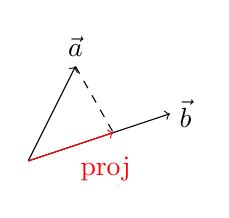
\begin{tikzpicture}[scale=0.6]
        \draw[->] (0,0) -- (3,1) node[right] {$\vec{b}$};
        \draw[->] (0,0) -- (1,2) node[above] {$\vec{a}$};
        \draw[dashed] (1,2) -- (1.8, 0.6);
        \draw[->, red] (0,0) -- (1.8, 0.6) node[midway, below right] {proj};
    \end{tikzpicture}
    \captionof*{figure}{Projection}
\end{minipage}%
\begin{minipage}{0.55\linewidth}
    \textbf{Projection of $\vec{a}$ onto $\vec{b}$:} \\
    $\text{proj}_{\vec{b}}\vec{a} = \frac{\vec{a} \cdot \vec{b}}{|\vec{b}|^2} \vec{b}$ \\
    \bn{ভেক্টর $\vec{a}$ এর ছায়া বা উপাংশ ভেক্টর $\vec{b}$ এর ওপর কতটুকু তা বের করার জন্য।}
\end{minipage}

\textbf{Cross Product:}
$\vec{a} \times \vec{b} = \begin{vmatrix} \hat{i} & \hat{j} & \hat{k} \\ a_x & a_y & a_z \\ b_x & b_y & b_z \end{vmatrix}$ \\
\bn{দুটি ভেক্টরের লম্ব ভেক্টর (Normal Vector) পেতে অথবা তাদের দ্বারা গঠিত সামান্তরিকের ক্ষেত্রফল (Area of Parallelogram) এবং ত্রিভুজের ক্ষেত্রফল ($0.5 \times |\vec{a} \times \vec{b}|$) বের করতে।}

\subsubsection*{Coordinate Geometry & Rotation}
\bn{একটি বিন্দু $(x, y)$ কে মূলবিন্দুর (Origin) সাপেক্ষে $\theta$ কোণে ঘড়ির কাঁটার বিপরীতে (Counter-Clockwise) ঘোরাতে:}

\textbf{2D / Rotation around Z-axis:} \\
$x' = x \cos \theta - y \sin \theta, \quad y' = x \sin \theta + y \cos \theta$

\textbf{Rotation around X-axis} ($x$ remains fixed): \\
$y' = y \cos \theta - z \sin \theta, \quad z' = y \sin \theta + z \cos \theta$

\textbf{Rotation around Y-axis} ($y$ remains fixed): \\
$x' = x \cos \theta + z \sin \theta, \quad z' = -x \sin \theta + z \cos \theta$

\textbf{Rodrigues' Formula:} (Rotation of vector $\vec{v}$ by angle $\theta$ around axis unit vector $\vec{u}$) \\
$\vec{v}_{rot} = \vec{v}\cos\theta + (\vec{u}\times\vec{v})\sin\theta + \vec{u}(\vec{u}\cdot\vec{v})(1-\cos\theta)$ \\
\bn{যেকোনো 3D ভেক্টরকে যেকোনো অক্ষ (Axis) সাপেক্ষে ঘোরাতে এটি সবচেয়ে পাওয়ারফুল সূত্র।}

\subsubsection*{Solid Geometry}
\noindent
\begin{minipage}{0.45\linewidth}
    \textbf{Sphere (গোলক):} \\
    $\text{Volume} = \frac{4}{3}\pi r^3$ \\
    $\text{Surface Area} = 4\pi r^2$
\end{minipage}%
\begin{minipage}{0.55\linewidth}
    \textbf{Cone (কোলক):} \\
    $\text{Volume} = \frac{1}{3}\pi r^2 h$ \\
    $\text{Surface Area} = \pi r(r + \sqrt{h^2+r^2})$
\end{minipage}

\vspace{0.5em}
\noindent
\begin{minipage}{0.45\linewidth}
    \centering
    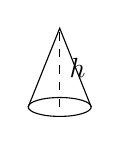
\begin{tikzpicture}[scale=0.4]
        \draw (0,0) ellipse (1 and 0.3);
        \draw (-1,0) -- (0,2.5) -- (1,0); 
        \draw[dashed] (0,0) -- (0,2.5) node[midway,right] {$h$};
    \end{tikzpicture}
    \captionof*{figure}{Cone}
\end{minipage}%
\begin{minipage}{0.55\linewidth}
    \textbf{Pyramid:} \\
    $\text{Volume} = \frac{1}{3} \times \text{Base Area} \times \text{Height}$ \\
    \bn{পিরামিডের আয়তন বের করতে ভূমির ক্ষেত্রফল জানা থাকতে হবে।}
\end{minipage}

\subsubsection*{Triangle Properties}
\textbf{Equilateral Triangle Area:} $\frac{\sqrt{3}}{4}a^2$

\textbf{Inradius ($r$):} $r = \frac{\Delta}{s}$ \quad \bn{($\Delta = $ ত্রিভুজের এরিয়া, $s = $ অর্ধপরিসীমা)} \\
\textbf{Circumradius ($R$):} $R = \frac{abc}{4\Delta}$ \quad \bn{($a,b,c$ হলো তিন বাহু)}

\textbf{Sine Rule:} $\frac{a}{\sin A} = \frac{b}{\sin B} = \frac{c}{\sin C} = 2R$ \\
\bn{ত্রিভুজের বাহু এবং বিপরীত কোণের সম্পর্ক। পরিবৃত্তের ব্যাসার্ধ বের করতেও লাগে।}

\textbf{Cosine Rule:} $\cos A = \frac{b^2+c^2-a^2}{2bc}$ \\
\bn{তিনটি বাহু জানা থাকলে কোণ বের করতে, অথবা দুটি বাহু ও অন্তর্ভুক্ত কোণ জানা থাকলে তৃতীয় বাহু বের করতে।}

\begin{center}
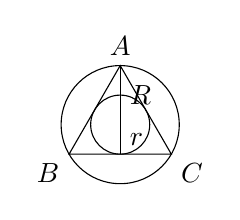
\begin{tikzpicture}[scale=0.5]
    \draw (0,0) circle (1.5);
    \draw (90:1.5) coordinate (A) -- (210:1.5) coordinate (B) -- (330:1.5) coordinate (C) -- cycle;
    \node at (A) [above] {$A$};
    \node at (B) [below left] {$B$};
    \node at (C) [below right] {$C$};
    \draw (0,0) -- (A) node[midway, right] {$R$};
    \draw (0,0) circle (0.75);
    \draw (0,0) -- (270:0.75) node[midway, right] {$r$};
\end{tikzpicture}
\end{center}

\subsubsection*{Number Theory}
\textbf{Divisors of $N = p_1^{a_1} p_2^{a_2} \dots$ :} \\
$\text{Count} = (a_1+1)(a_2+1)\dots$ \\
$\text{Sum} = \prod \frac{p_i^{a_i+1}-1}{p_i-1}$

\textbf{Logarithm:} $\log_b x = k \iff b^k = x$ \\
$\text{Number of Digits in Base } b = \lfloor \log_b(N) \rfloor + 1$ \\
\bn{যেকোনো সংখ্যার ডিজিট সংখ্যা বের করার শর্টকাট।}

\subsubsection*{Linear Algebra (Cramer's Rule)}
\bn{দুই চলক বিশিষ্ট সরল সমীকরণ সমাধান করতে:} \\
System: $ax+by=e, \; cx+dy=f$ \\
$D = \begin{vmatrix} a & b \\ c & d \end{vmatrix} = ad-bc$ \\
$D_x = \begin{vmatrix} e & b \\ f & d \end{vmatrix} = ed-bf, \quad D_y = \begin{vmatrix} a & e \\ c & f \end{vmatrix} = af-ce$ \\
Answer: $x = \frac{D_x}{D}, \quad y = \frac{D_y}{D}$ \quad (Valid if $D \neq 0$)
